% Introduction
% If your a planing to contribute to this documentation, then please create 
% for every major "chapter" a new file with an meaningfull caption and add it 
% to this file using the "\input{<caption>}" function



\documentclass{acm_proc_article-sp}
\usepackage[utf8]{inputenc}
\usepackage[T1]{fontenc}
\usepackage[english]{babel}
\usepackage{amssymb} % set symbols i.e. /mathbb{N}
\usepackage[colorlinks=false, pdfborder={0 0 0}]{hyperref}
\usepackage{listings}
\usepackage{graphicx}

%Bibliogr.
\usepackage[numbers]{natbib}
\bibliographystyle{acm}

\begin{document}

%what is the corret title again?
\title{Documentation - Urban HCI\\Distributed Klick/Flickable Interfaces for Public Spaces}
%\subtitle{Subtitle}


%please check for the right number of authors
\numberofauthors{3}

%use to given format to add yourself as a author
\author{
  \alignauthor 
   Daniel Pollack \\
   \affaddr{Medieninformatik Bc.}\\
%   \affaddr{Matrikelnr.: 100488}\\
   \email{daniel.pollack@uni-weimar.de}   
   %
   \alignauthor 
  Jenny Gonzalez\\
   \affaddr{Computer Science and Media M.Sc. student}\\
%   \affaddr{Matriculation number: 112442}\\
   \email{jenny.carolina.gonzalez.\\acuna@uni-weimar.de}    
  \alignauthor 
   Ingo Schäfer \\
   \affaddr{Medieninformatik Bc.}\\
%   \affaddr{Matrikelnr.: 100488}\\
   \email{ingo.schaefer@uni-weimar.de}   
} 

     
\date{\today}

\maketitle

\section{ABSTRACT}
The project described in this work consists of a network of wireless nodes with a star topology. The main node is constituted by two entities: a computer with a Java-based server and a panstamp device, both of them interconnected. The rest of the nodes are divided into two types: sensor and actuator nodes; the former gathers information and sends data to the main node while the latter receives data from the main node and reacts to it accordingly. The Java-Server manages all network nodes depending on the recollected data, and provides an interface to allow users the configuration of different settings in the network. With the interface, users can create their own setups and get a quick and complete overview of the network status.The sensor and actuator nodes are grouped in pairs to form independent entities in the network and each one
of these entities reacts differently to each possible situation. The Java-server determines the personality of each entity. 

\section{Related Work}
The target of this project was to create a newly kickbale and flickable interface used in the outside. For that we firstly did some researches in the web getting inspirated for what we could do.
At least, we hadn't used those literature we had found because there was no interface that can be kicked.
 
\subsection{Listening Lanterns}
The idea of this project was to create a kickable interface for the outside. One of our first findings, was a bubble changing its colour by holding it. The idea of those people was to create a new portable device lightning up your way home in the dark. Firstly, in the middle ages, each person used its own lantern. Later, in the beginning of 18th century some cities like Paris started to lighten their streets at night. They wanted to go back and give each person an own personnel light. So each of those lanterns had an own specifying colour and a fading pattern.\newline
With this basic idea, they started to implement new ideas. \newline

\subsection{DJ Light}

\begin{figure}[h!]
	\centering
	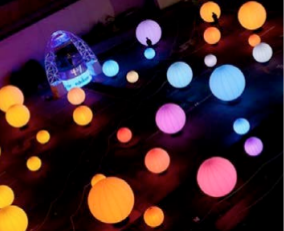
\includegraphics[width=0.5\textwidth, clip=true, keepaspectratio=true]{./pic/dj_light.png}
	\caption{DJ Lights}
	\label{fig:DJ_Lights}
\end{figure}

Using that lantern idea, another team created a public sound and light installation.\newline
They built several sphere - formed devices which can change their colour by different auditive input. With this technology, visitors can perform an own orchestration. Because there are many spheres, the installation can be transported and reinstalled relatively simple. So the devices are pretty good for a usage in the outdoor.\newline
This idea of multiple small devices we used to. \newline 
http://www.wordlesstech.com/2011/01/16/dj-light-installation-video [09.09.2013, 13:50]\newline

\subsection{Throwable Interfaces}
Another very interesting project was to built sticky LED candles which can be threw onto a wall where they rest. After that, an interacting person can target one of those candles with a laser remote. When they get targeted, they changed their color. \newline

\subsection{Urban Cursor}

\begin{figure}[h!]
	\centering
	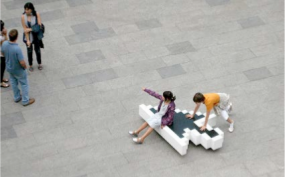
\includegraphics[width=0.5\textwidth, clip=true, keepaspectratio=true]{./pic/urban_cursor.png}
	\caption{Urban Cursor}
	\label{fig:urban_cursor}
\end{figure}

Another urban hci - project we recognized was the Urban Cursor.\newline 
Here, a team created a furniture, designed like a cursor. Approximately, its size is about two to three square metres. The whole thing is easy moveable, because of its wheels. The feature of the cursor is the GPS - tracking system. So the team could determine how the passers - by moved the furniture through the urban space.\newline
The cursor has a very large size because merely people should use it together, so that the project has a social aspect to.
http://www.urbancursor.com [09.09.2013] 

\subsection{Pixels Light Installation}

\begin{figure}[h!]
	\centering
	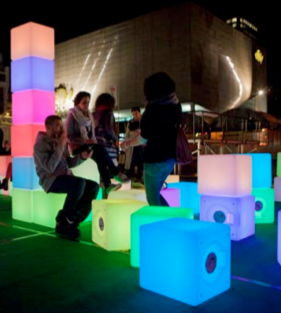
\includegraphics[width=0.5\textwidth, clip=true, keepaspectratio=true]{./pic/pixels_light_installation.png}
	\caption{Pixels Light Installation}
	\label{fig:pixels_light_installation}
\end{figure}
Here the designers built merely cube - devices. \newline
The idea was to built an installation similar to lego \texttrademark where a user can put those devices together or stack them to built different constructed forms. \newline
The cubes are color and intensity changing by rotation. Beyond that, each of the devices is direct and wirelessly connected to the others. So the environment is not driven by a server - client - system.\newline
By using the Arduino technology, those devices are using RF - and IF - sensors, so that they can recognize each other. So when they got kinetic input they will change their colour. With the connection the installation recognizes when some devices are put together, then the construct can be lighten up just in one colour. (All cubes are changing to that one colour.)\newline
 Furthermore the cubes are waterproof, so they can be used in the outside.\newline
\newline
http://www.lightpublic.com/lighting-articles/get-pixelated-with-the-pixels-light-installation [09.09.2013] \newline

\subsection{Liquid bricks}

\begin{figure}[h!]
	\centering
	
\includegraphics[width=0.5\textwidth, clip=true, keepaspectratio=true]{./pic/liquid_bricks.png}
	\caption{Liquid Bricks}
	\label{fig:liquid_bricks}
\end{figure}
 
This was a small urban project about a water - filled pouch. \newline
The idea was to built any furniture which can be used to make a fun for the passers - by. With this the team designed a texture seeming like the street's bricks. After that, they put the pouch to the ground - level of the street / square. So when a person was walking over it, it seemed like walking over a inconsistent place.\newline
\newline
http://www.thisiscolossal.com/2011/06/liquid-bricks\newline

\subsection{21 swings}

\begin{figure}[h!]
	\centering
	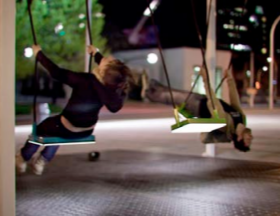
\includegraphics[width=0.5\textwidth, clip=true, keepaspectratio=true]{./pic/21_swings.png}
	\caption{21 Swings}
	\label{fig:21_swings}
\end{figure}

In Montreal a gigantic wings installation was created along a street.\newline
By swinging on a swing a music note is played. So when just one lonely passer - by is swinging, the system doesn't makes that fun. But when merely users are in action with the swings a hazard harmonic is in creation. \newline
Here the designers used the diatonic music system. This is the system which is known from playing harmonica: When the user is blowing in one specific hole, a tone will sound. When the user is suck in the same hole, the next tone in the musical scale will sound. Here in this project, each swing just gives one tone. It doesn't matter if the swing is swinging back- or forwards. The clue on this pattern is, that there cannot be any false note which doesn't match to the others.\newline
\newline
http://www.fastcodedesign.com/1672192/watch-a-musical-swingset-forms-a-21-piece-orchestra.                

\section{Concept}

\subsection{Basic Concept}
The basic concept for this project was to create a interface, which is modular and mainly mobile. Like already explained we wanted to create a interface that has more degrees of freedom in terms of the usage than a installation which is bound to a place and therefor mobile. Due to the fact that we decided to use a more powerful server to manage all devices, we reached a certain degree of bounding to a place, while still being mobile. 

\subsection{Hardware Concept}
%hardware, advantages of microcontrollers, engery problems, wireless stuff

\subsection{Software Concept} 
To achive the degree of mobility, the server only needs a connected panstamp to work properly. It is also possible to put the server software on a more powerful microcontroller like a raspberry pi or some similar controller.
The modularity is given through a number of easy configurable files. Changing behavior, apperance or the defined actions is pretty easy to do.


\section{Development}
The creative process of finding an idea how to create something ''kickflickable'' began with a small introduction to arduino. Mainly we were thought the workflow and usage of an arduino, and therefor of an microcontroller in general, by the lady ada tutorial. \cite{lady_ada_arduino_tutorial}
We learned how to use basic components like LEDs and tilt-sensores. Very early we recognized, that sensores for position measurement were needed to recognize the position of the future device. But we also experimented with a skate-wheel to for example wether it turns one way or the other. To make sure that the finished prototypes and the concept are expandebel in terms of new sensors and/or actuators.
After we found the right sensors we needed to find a way to communicate with the devices. We experimented with panStamps \cite{panstamp} and XBee\cite{xbee}-shields. In the end we settled with the panStamps because of their larger range results and the fact of them combining a arduino with a wireless module to one device instead of additionally getting one more interface to work on.

Form this point on, we had an idea of how to realise the position detection and communication parts. We still needed to create some sort of feedback for the user to realize. 
At first we wanted to give feedback via audio, vibration and light, but because of limitations in time and processing power of the ATmega %cite genauer bautyp
 chip we decided to keep the most obvious of the three feedback ideas and settled with the light.

The finished prototypes now run on two panStamps with a ATmega<bla> each. On panStamps controlls the sensors and the other is meant to create the feedback. 
A RGB LED Chain was selected to create light patterns, because of the convenient usage and the brightness of the LEDs. 

% vim: spell spelllang=en_gb 

\section{The Java Server}

\subsection{First development steps}
As explained in the Software Concept section, the Java server receives from the server node all the data gathered in the network, produces a response according to each module’s personality and sends the corresponding commands to the intended actuator nodes through the server node.

To develop the Java server, we first divided its envisioned structure into subcomponents and worked with each part at a time. The first subcomponent was a serial port communication system, the second was the graphical user interface. Later, we learned about threads and runnable concepts in Java to implement another subcomponent dedicated to the management of the different nodes in the network. 

As a first step, we implemented a basic serial port communication routine for learning and experimenting purposes. For this, we worked with the RxTx-library to get a better understanding of the tools it provided. The small application only wrote information to the serial outputstream and if there were available data coming from the serial port, it read the data and printed them in the console.

After understanding the ground principles of the library, we began to design and implement the Java server.



\subsection{Graphical User Interface}
\subsubsection{Main Window}
The User Interface is meant to provide the user with all necessary informations about the registered devices without showing to much information at once. Therefore the main window consists of two parts. 
The first part is form connecting and disconnecting the server panstamp. While attempting to establish a connection, the users can select every serial port with an attached device as well as the baut-rate. Once the Java-Server is connected, the Connect-Buttons label changes it's text and turns into a Disconnect-Button. This option is accessable at all times, so that the user can disconnect/reconnect at any time. For example if one decides to change the used serial port. 
If the server did not recocnise a device on any of the serial ports. The connect button will be unavailable. This is realized through disabling the button. To prevent the user from constantly restarting the server, we implemented a refresh button, which can be pressed at any time and if this time a device on one of the serial ports was detected it/they will be displayed in the according combobox for selection and connection.


The second part displays a table of all the known devices, their state and a timestamp as well as their personalities name. This table updates itself with a fixed frequency, to ensure that for example every new device and/or every change in state is visible to the user. The update process was realized through a timed task provided by the swt-library. The frequency is configurable. More information in the interface architecture section. %insert link here

\begin{figure}[h!]
 \centering
 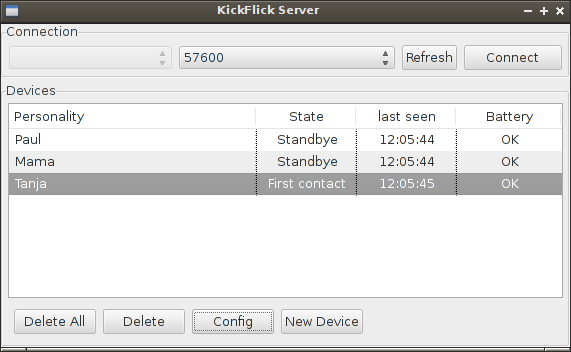
\includegraphics[width= 0.5\textwidth, clip=true  ,keepaspectratio=true]{./pic/java-server-main.png}
 % java-server-main.png: 0x0 pixel, 0dpi, nanxnan cm, bb=
 \caption{Main Window}
 \label{fig:java-server-main}
\end{figure}



If the server got at least one device, the user can select it in the device-table and open a configuration dialog by pressing either the configuration button, on the bottom of the table, or double clicking on the selected table item. A configuration dialog will then open, were this particular device and its personality can be altered.

\subsubsection{Configuration Dialog}
Once the user decided to configure on device, this dialog opens and provides him, on three tabs, with all the necessary informations and options to configure the device and its personality full scope. %anders formulieren%

The user can decide whether he wants use a preconfigured personality for this particular device or not. A preconfigured personality will, if selected, change all settings to its own settings and thereby overwrite, temporarly, ale previous settings. No matter how the users decides, he can then begin configuring the device and personality. The configuration process can be determinated every time by pressing the operation systems colse button in one corner of the dialog window. No settings will then be written.

On the first tab, labeled ''Basic'', the basic informations like the name of the personality and the addresses of both nodes are shown. Below the user finds a table with all known action keys, and whether the device will react to this particularly key or not. The reaction willingness is hereby represented by a checkbox showing a hock, if a reaction will happen and no hock when there will be no reaction to this key. The user can change every key value as he wishes.

\begin{figure}[h!]
 \centering
 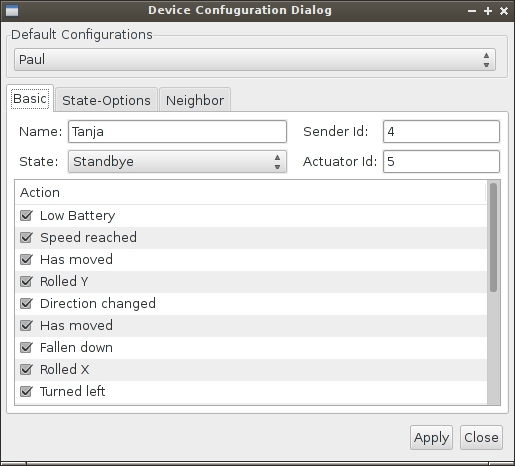
\includegraphics[width= 0.5\textwidth, clip=true  ,keepaspectratio=true]{./pic/java-server-config01.png}
 % java-server-main.png: 0x0 pixel, 0dpi, nanxnan cm, bb=
 \caption{Configuration Dialog, 1st Tab}
 \label{fig:java-server-config01}
\end{figure}

The second tab shows in a checkbox the current state of the device. The state can be changed by the user. Below the checkbox a table with all seperate states of the personality is shown and one can change the pattern and both colors for a particular state. 


\begin{figure}[h!]
 \centering
 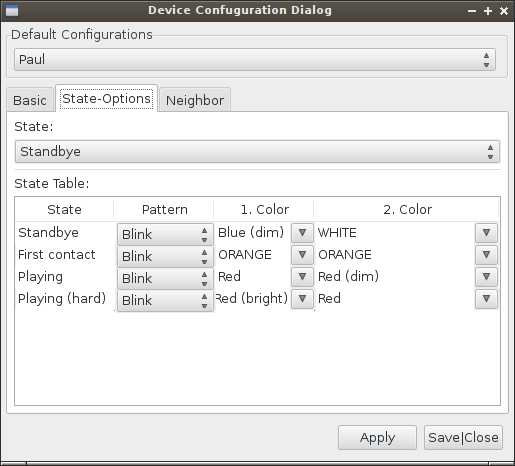
\includegraphics[width= 0.5\textwidth, clip=true  ,keepaspectratio=true]{./pic/java-server-config02.png}
 % java-server-main.png: 0x0 pixel, 0dpi, nanxnan cm, bb=
 \caption{Configuration Dialog, 2nd Tab}
 \label{fig:java-server-config01}
\end{figure}


The third tab displays the actions performed when a neighbor is detected. The table shows every known personality, known by the server at this time. Except for the preset personalities. The preset personalities already know their reaction to the other preset personalities, even if they are yet unknown by the server.
The user can once again configure the pattern and colors of this neighbor reaction. Those settings will then be transmitted to both devices, the one who noticed the neighbor and the neighbor.

After the user finished the configuration and wants to write the new settings to the device, he will need to first press the apply button and then the save and close button to actually writhe the settings. Otherwise if just the save and close button was pressed, no changes will be written and the device remains like before the configuration process.
\begin{figure}[h!]
 \centering
 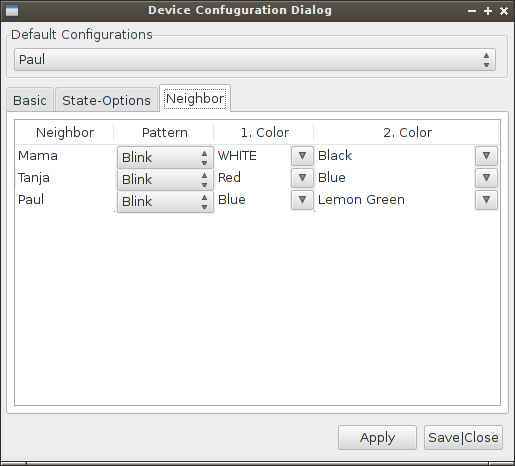
\includegraphics[width= 0.5\textwidth, clip=true  ,keepaspectratio=true]{./pic/java-server-config03.png}
 % java-server-main.png: 0x0 pixel, 0dpi, nanxnan cm, bb=
 \caption{Configuration Dialog, 3rd Tab}
 \label{fig:java-server-config01}
\end{figure}

\subsubsection{Interface Archticture}
The inferface was realised with the swt widget toolkit from eclipse. %insert cite
The main window uses a swt timerevent to periodicly update the device table. Every eventbased action, like button clicks or selection were also realized with the build-in eventlistener structure of the swt toolkit. %insert cite again

When the dialog is opened, the device will be passed as a parameter in the constructor, the dialog will then create the interface and afterwards read the settings of the device. 
The configuration will have no effect on the device at all, except the user says so. All changes will only be written when the apply button is pressen and even then a temporally device will be created to first save all settings in the instance


% vim: spell spelllang=en_gb 

\subsection{The Server}
The heart of the communication is the server. We chose java\cite{java} as our
programming language because of its multi platform abilities and the development
suit of eclipse\cite{eclipse} called swt\cite{swt} as our window-builder
framework.%need to rephrase this Except for one library, the
RxTx-Library\cite{rxtx}, we only used basic java libraries which came by default
with the eclipse IDE\cite{ide} environment; in other words, the
jdk7-openjdk\cite{open_jdk} package. %The heart of the communication is the server?

When the Panstamp server is connected to the Java server, the latter takes the data given by the Panstamp server thanks to the RxTx library \cite{rxtx} and passes the information to the parser for processing. %Each message is processed in a different thread, right?

%Provided that the user connected through the interface with a serial It takes most of the information broadcasted by the panStamps\cite{panstamp} and processes them.
%Provided the users connected through the interface with a serial port with the server-panStamp plugged in, the server takes the message with help of the RxTx-library %on a separate thread and passes the message, after receiving it, to the parser for processing and deciding.

The server checks with an external timed thread the state of each known device.
This thread checks the current state of the device and, if necessary, sets the
state back to standby if to much time since the last change has passed. Therefor
the thread compares the timestamp of the last state change with the current
time. Furthermore it checks if the neighborhood relationship is still existing
or not.

\begin{figure*}[ht]
	\centerline{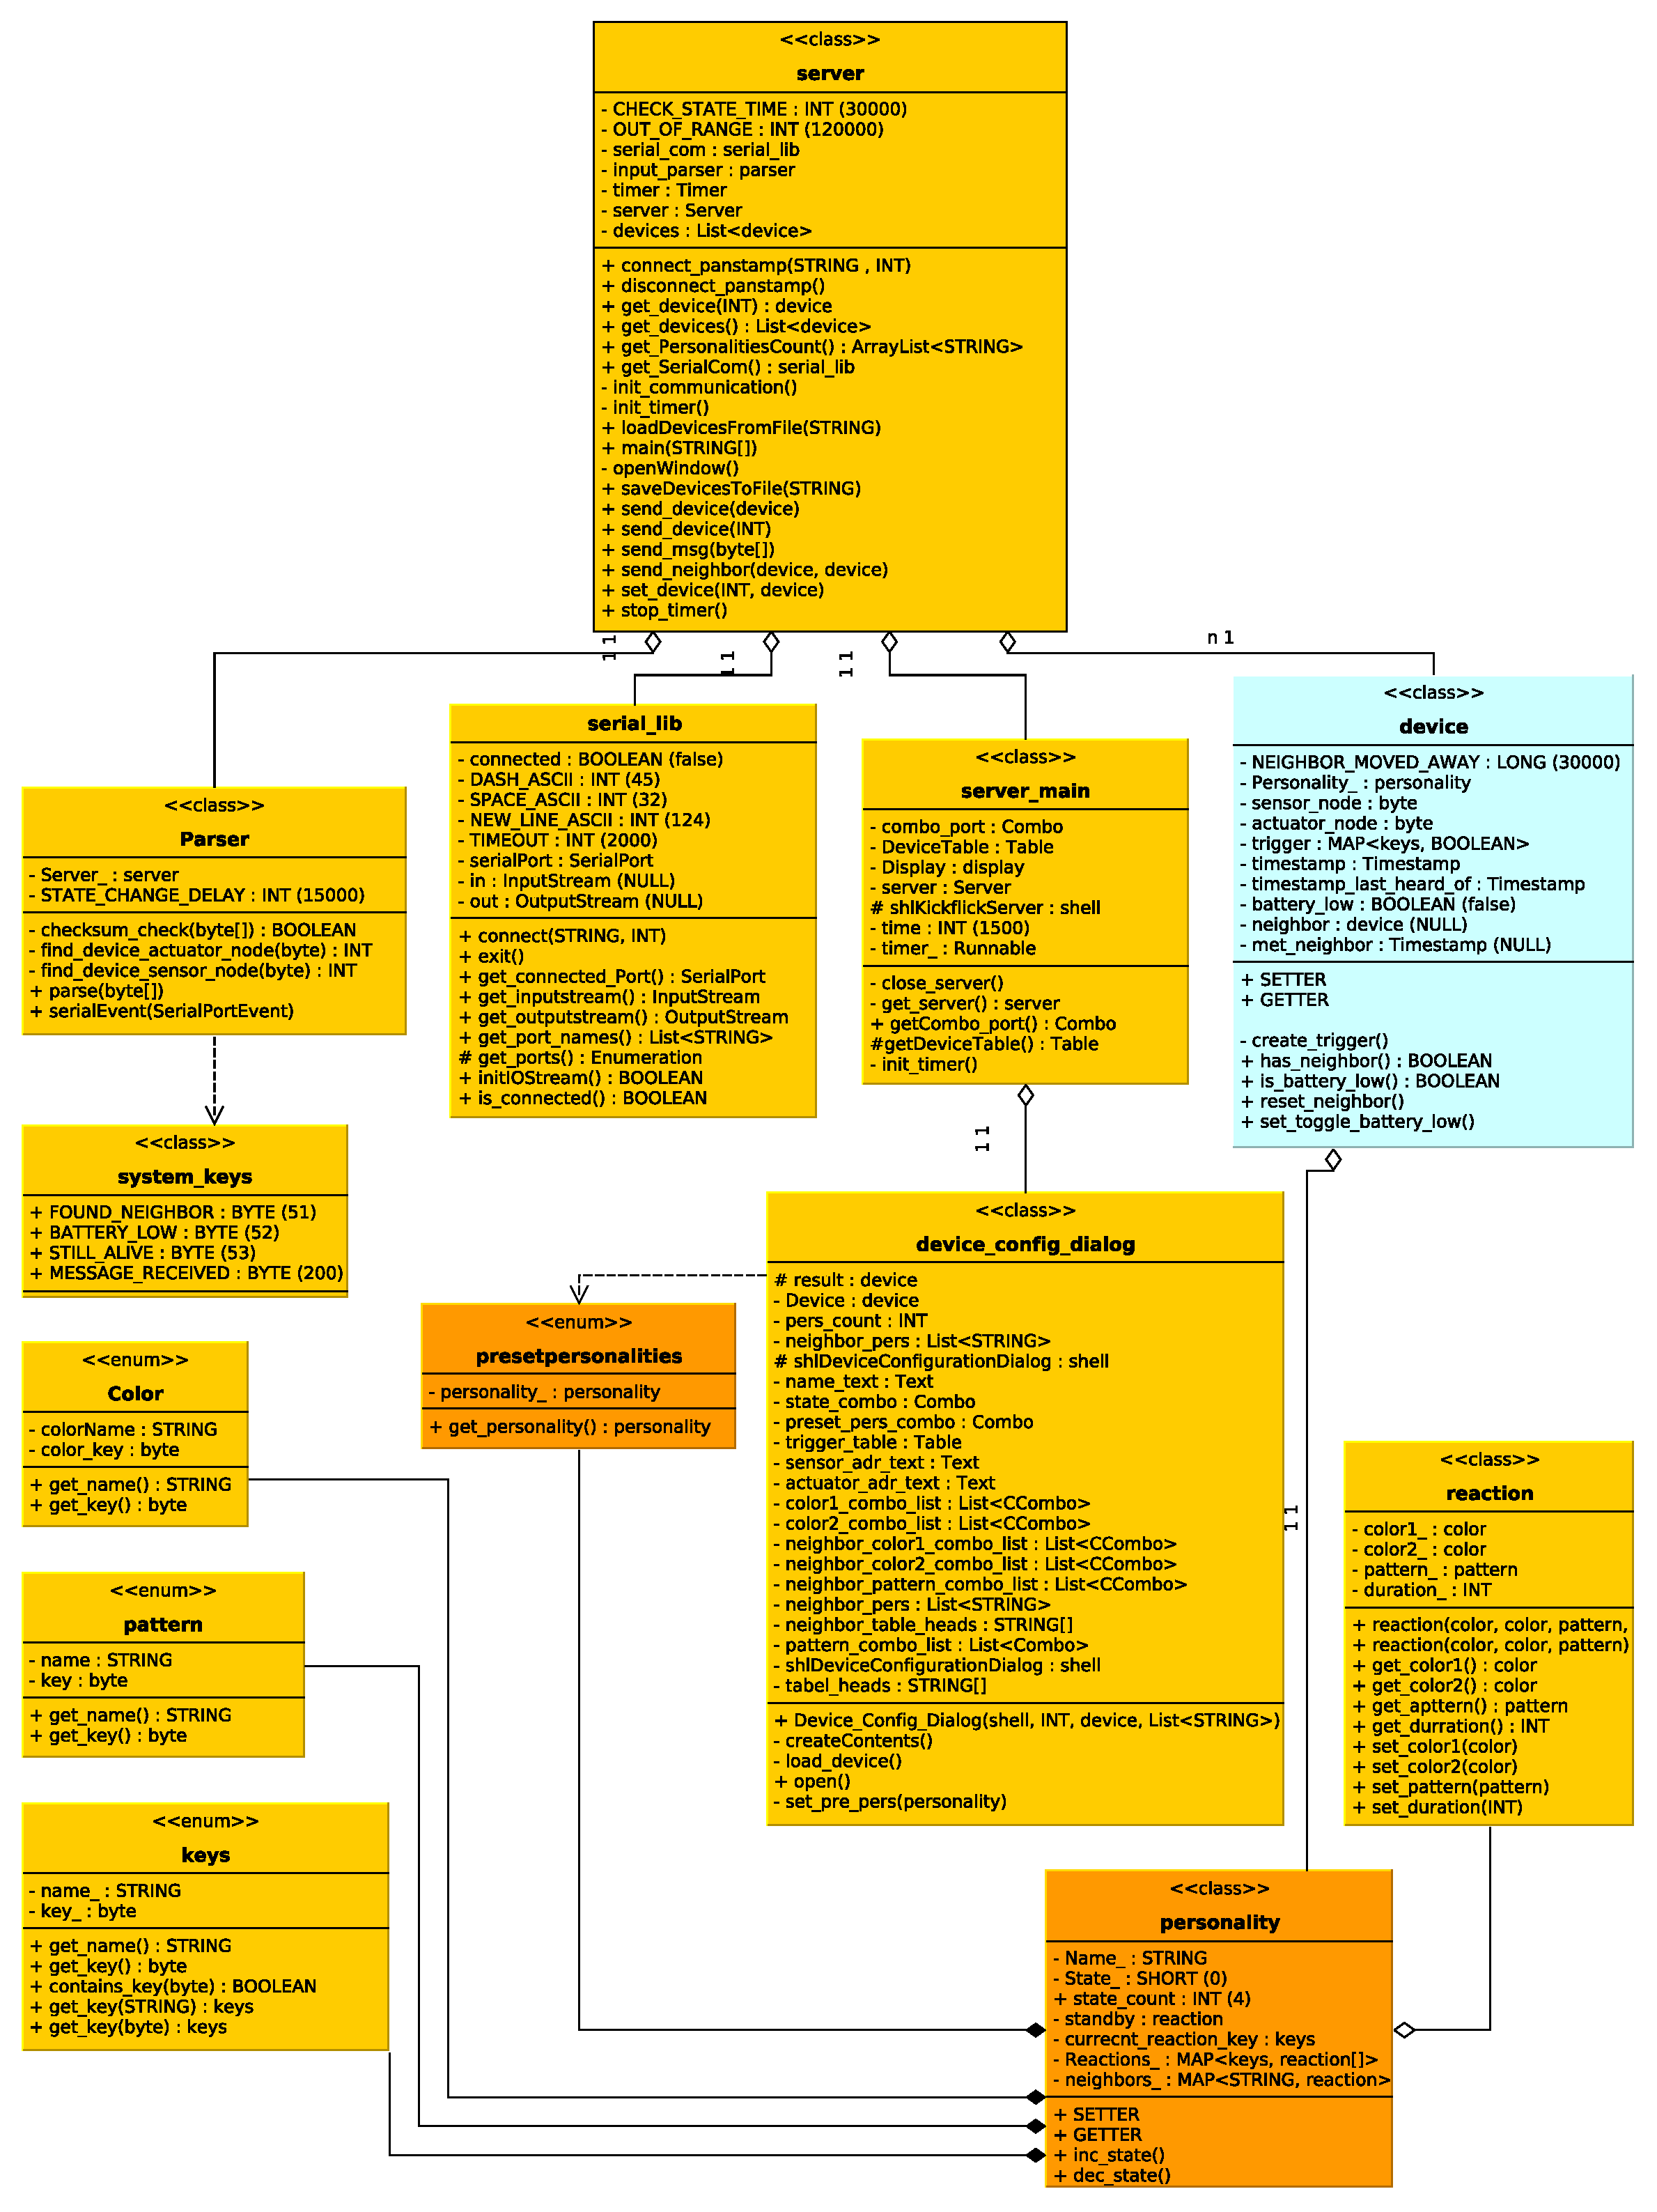
\includegraphics[width=\textwidth]{./graph/general.pdf}}
	\caption{UML Diagram of the Server Structure}
	\label{fig:server_uml}
\end{figure*}


\subsubsection{Panstamp-to-Java server message}
All messages sent by the Panstamp server to the Java Server contain four bytes. The message's length was set to a single value to achieve a better communication work-flow and to limit the communication's traffic to a minimum. Table~\ref{Panstamp-to-Java} shows the general structure of a message.


\begin{table}[h]
  \centering
  \begin{tabular}{ c | c | c | c }
    \hline
    \textbf{Byte 1} & \textbf{Byte 2} & \textbf{Byte 3} & \textbf{Byte 4} \\ [0.5ex]    
    \hline
    Sender's & Admin & Neighbor's Id| & Checksum  \\
    Id & Key & Dummy & \\
    \hline
  \end{tabular}
  \caption[Pamstamp-to-Java]%
          {Panstamp-to-Java server message's structure}
  \label{Panstamp-to-Java}
\end{table}

\begin{itemize}
\item \textbf{Sender's Id} is the Id of the network node that wants to report an event
\item \textbf{Admin Key} indicates the event reported by the entity. See table~\ref{Admin Keys} for further information.
\item \textbf {Neighbor's Id | Dummy } When the Admin Key equals NEARNODEEVENT, this byte contains the Id of the found neighbor node. For other keys this byte is ignored
\item \textbf {Checksum} This byte is the sum of bytes 1, 2 and 3 (modulo 256)
\end{itemize}

Table~\ref{Admin Keys} displays all the possible Admin Keys:

\begin{table}[h]
  \centering
  \begin{tabular}{ c | c }
    \hline
    \textbf{Name} & \textbf{Value}\\ [0.5ex]    
    \hline
    Shake Event & 31 \\
    Kick Event  & 32 \\
    Near Node Event & 51\\
    Low battery & 52\\
    In Range & 53\\   
    \hline
  \end{tabular}
  \caption[Admin Keys]%
          {Admin Keys}
  \label{Admin Keys}
\end{table}

\begin{itemize}
\item \textbf {Shake Event} indicates the entity has been shaken slightly so it is swaying
\item \textbf {Kick Event} means that the entity has been kicked or moved with a strong blow
\item \textbf {Near Node Event} signifies the entity has detected another entity which is really close to it
\item \textbf {Low Battery} warns the server that the entity's battery has to be recharged as soon as possible
\item \textbf {In range} indicates the server that the entity is still in range
\end{itemize}




\subsubsection{The Parser}
 
First, the parser checks whether the length of the package is exactly four bytes
and if the last byte, which is supposed to be a checksum summing the byte values
of every other byte in the message, matches the checksum calculated by the
server. If everything is correct the parser then searches for a known device in
the device list of the server, if it found no match it will create a new device
with default settings, otherwise the parser takes the found device and procede,
otherwise the parser takes the found device and procedess. , otherwise the
parser takes the found device and procedes. Once a device was found or created the parser begins to compare the second byte of the message for matching keys stored by the server. First all system\_keys will be compared. For example if the received message contains a ''52'' as second byte, the parser will then recognize this as the ''the battery is low'' key and will toggle the boolean value battery\_low of the device to true. 
If no system key matched with the received one, the parser then checks the
reaction keys of the device itself. This check only happens if the device it not
currently engaged in a neighborhood relationship with another device and if the
time of the last received state changing message lays back a certain time. For
this checking and comparing procedure the device owns a map with all reaction
keys stored to it and a associated boolean value, representing the choice of
ignoring or reacting to the received key. If a appropriate key was found and
according to the boolean value a reaction should happen, then the state of the
devices personality will be increased and the new information about the pattern
and both colors, depending on the received event key, will be send to the
server-panStamp using the RxTx-library. 

No matter if a correct message lead to a state change or not, the device will
get a new timestamp to memorize the time of the last received message. If a
state change happend the device also gets a new timestamp revering to the time
the last state change happend.

\subsubsection{Device and Personality Structure}
The server itself and the according class holds a list of all known devices. Every lookup action depends on this list. The device class itself holds a instance of the personality class.
Devices can be seen as a representation of the hardware devices with the two panStamps in them. It refers to the hardware and therefor stores the Id's of the panStamps and timestamps of the last received message either one of the hardware device panStamps, a second timestamp of the last state change and a third timestamp of the last ''neighborhood meeting''. All those information are accessible through ''get'' functions as well as mostly modifiable through ''set'' functions.

The personality stores the reaction of a particular device depending on the
event keys, neighbors and the state of the device. For the purpose of reaction
to a certain event key the personality stores
a map for reactions with the acording keys as key and an array of reaction class
instances. If for example the parser received a message with an event key, the
reaction map will be searched for this particular key. If this key exsists in
the map the reaction array will be returned and the personality returns the
proper reaction fitting the current state. If the map holds no entry for the
gven key, the reaction map returns a default reaction array from with a fitting
reaction acording to the state will be returned. For this matter the default
map structre was extended to fit those requirements.
The possible reactions to each neighbor personality is also stored in a map. This
map contains the name of the personality as a key and one reaction as value. 
%The personality class stores information about the states of the personality and the according patterns and colors. This class also provides ''get'' and ''set'' functions to retrieve or change values. Additionally the personality class stores map object of all known personalities and the appropriate response in form of pattern and colors to every possible neighbor. If the device and therefor the personality encounter a unknown personality as a neighbor a default response will be send. 
%The neighbor map provides the ability to set reactions to neighbor personality, even if they don't exist yet.

Reactions represened by a class called reaction. This class stores information
about colos, patterns and the duration of one reaction. The duration determines
the time a reaction will be at least visible on the hardware.

To get the server and the project running without setting up every single device
by hand a enumeration for pre defined personalities was created. One can select
between each of those personalities. Once a pre defined personality is selected,
the previous personality of the current device will be overwritten. This
approach saves time. It is also possible to save the current devices to a file
so that they can be loaded again, for examlpe after restarting the server.
Therefor the classes device, personality and reaction are extending the
serialize class.

\subsubsection{Key Structure}
During the development we thought of keys, single byte values, to represent commands, messages, patterns and colors. To store these keys several enumerations were created to seperate related keys with their name and value depending on their usage.
We divided the keys in enumerations:
\begin{itemize}
    \item system
    \begin{itemize}
         \item stores basic keys for transmitting status information (e.g. ''low battery'')
				 \item enumeration: system\_keys
    \end{itemize}
    \item color
    \begin{itemize}
        \item stores byte values for every color hard coded to the actuator panStamp of the hardware device
				\item enumeration: color
    \end{itemize}
    \item pattern
    \begin{itemize}
        \item stores byte values for every pattern hard coded to the actuator panStamp of the hardware device
				\item enumeration: pattern
    \end{itemize}
    \item event key
    \begin{itemize}
        \item stores byte values for every possible action happening to the hardware device
				\item enumeration : keys
    \end{itemize}
\end{itemize} 

Every class or function referring to those values calls only the enumeration item by its name. The advantage of this approach is easier changing of single values as well as a quicker overview.




\section{driver}
The Panstamps' drivers were completely made in C++. Each different node in the network, namely server, actuator and sensor node, has its own driver; nevertheless, all of them are based on the class "node". 
\section{Hardware}
\subsection{Sensor Node}
The sensor node is constituted by the panstamp, an accelerometer and a voltage divisor circuit.

\subsubsection{Accelerometer}
\label{sec:Accelerometer}
The ADXL335 is a small low power 3-axis accelerometer that measures acceleration with a range of at least +/- 3g; in other words, +/- 3g is the maximum amplitude that this accelerometer can detect before distorting or clipping its output signal. 1g is the acceleration due to the earth's gravity (9.8 m/sec2).

According to the ADXL335 datasheet (add reference), the capacitors Cx, Cy and Cz connected to the accelerometer pins Xout, Yout and Zout determine the accelerometer's bandwidth. With these capacitors, a low pass-filter for anti-aliasing and noise reduction is implemented. Aliasing denotes the distortion and artifact that can appear when a signal is reconstructed from samples of the original signal (see reference XX and section~\ref{sec:Accel class}). In the board GY-61 (see Figure~\ref{fig:accelerometer}), Cx, Cy and Cz have a capacitance of 0.1uF that yields a bandwidth of 50 Hz (add reference). 	

\begin{figure}[h!] 
 \centering
 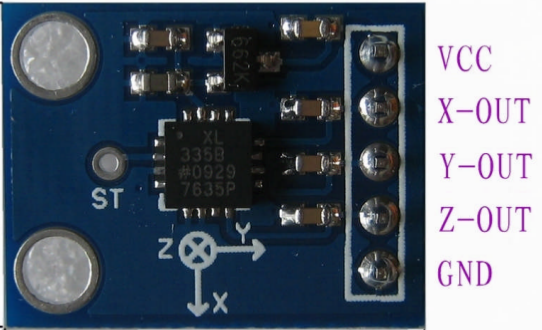
\includegraphics[width= 0.35\textwidth, clip=true,keepaspectratio=true]
 {./pic/accelerometer.png}
 \caption{ADXL335 accelerometer in board GY-61}
 \label{fig:accelerometer}
\end{figure}  
    
  
\subsubsection{Voltage monitoring circuit}
\label{sec:Voltage monitoring circuit}
To detect when the Li-Po battery has low voltage, a voltage monitoring circuit was implemented with the Panstamp's analog comparator module (add reference to the data-sheet here) and a voltage divisor circuit (see Figure~\ref{fig:voltage-monitor}). According to the ATMEGA 328 data-sheet (add reference), the Analog Comparator compares the input values on the positive pin AIN0 and negative pin AIN1. 

In our implementation, the Analog Comparator triggers an interruption in the sensor node when the voltage on the pin AIN0 decreases below the voltage in pin AIN1. With the configuration shown in Figure~\ref{fig:voltage-monitor}, the voltage in AIN1 is always 2.4 V. When the Li-po battery voltage falls below 9.5 Volts, the voltage in AIN0 (which is the same voltage in resistor R2) is less than the voltage in AIN1 and the Analog Compator activates as a result an interruption.

To minimize power dissipation in the voltage monitoring circuit, the possible maximum current in brach R1-R2 and in branch R3-R4 was fixed to 0.1mA. With this value and the maximum voltage given by the Li-po battery (12.5 V) the values of R1, R2, R3 and R4 were calculated.  

\begin{figure}[h!] 
 \centering
 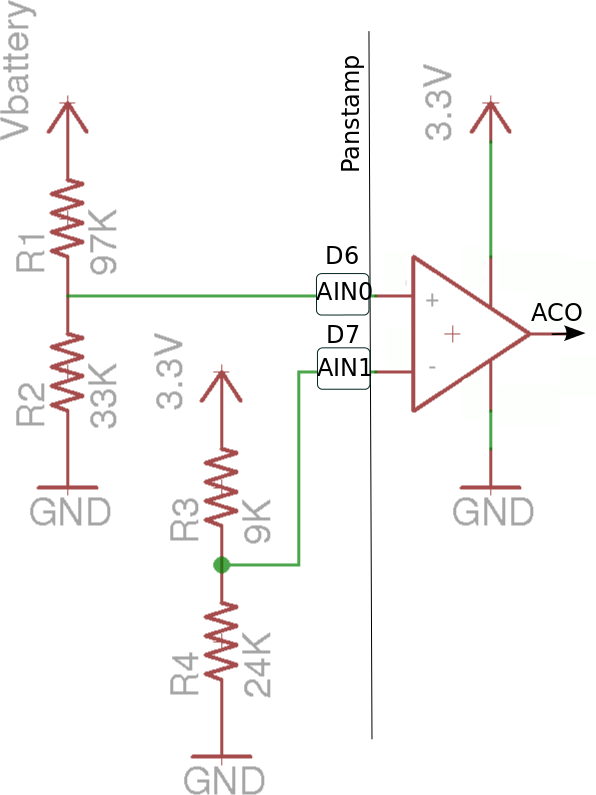
\includegraphics[width= 0.35\textwidth, clip=true,keepaspectratio=true]{./graph/voltage_comparator_circuit.png}
 \caption{Voltage monitoring circuit}
 \label{fig:voltage-monitor}
\end{figure}

\subsection{Actuator Node}
The actuator node is constituted by a panstamp and a led strand, whose length varies among the different modules. 
\subsubsection{Led strand}
In the led strand, each pixel contains a small microchip called LPD6803 and both led and chip are encapsulated within a silicone enclosure . Thanks to this microchip, each pixel in the strand can be controlled individually. It is recommended to use a supply voltage of 5 volts for the led strand (See LPD6803 datasheet). As shown in Figure~\ref{fig:led-strand}, the led strand has 4 cables: the red and white ones are for the power supply (red is positive and white has to be connected to ground), the blue one is the data cable and finally the green one is the clock cable. In our system, blue is connected to the panstamp's digital pin 5 and the green cable is connected to the panstamp's digital pin 3. 

\begin{figure}[h!] 
 \centering
 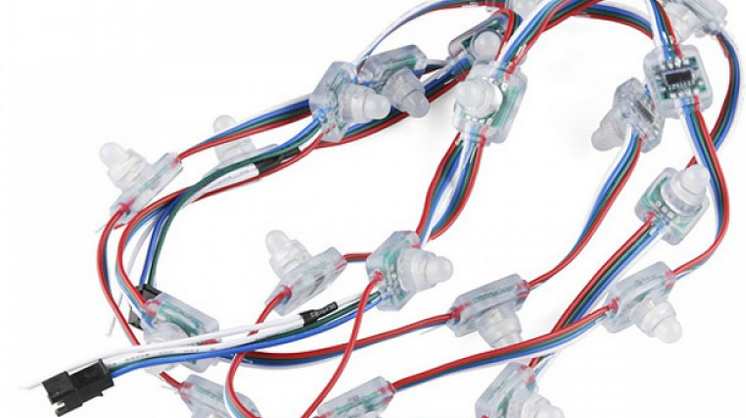
\includegraphics[width= 0.35\textwidth, clip=true,keepaspectratio=true]{./pic/led-strand-all.jpeg}
 \caption{Led strand}
 \label{fig:led-strand}
\end{figure}

\subsection{Server Node}
The sensor node is constituted by a panstamp and a panStick (See Figure~\ref{fig:panstick}).
PanStick is a USB mother board that enables both the programming of panStamps and the communication between a panstamp and a computer via USB.

\begin{figure}[h!] 
 \centering
 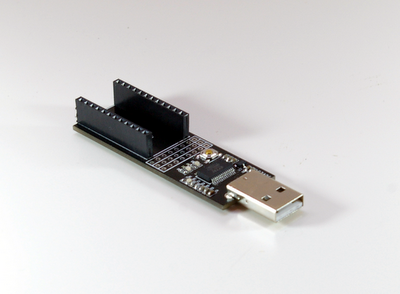
\includegraphics[width= 0.35\textwidth, clip=true,keepaspectratio=true]{./pic/panStick_01.png}
 \caption{Panstick}
 \label{fig:panstick}
\end{figure}

Additionally, the panStick includes a reset button that lets restart an application without having to unplug the board. 
\section{Miniproject: The wheel}
\label{sec:the-wheel}
Before the main project's goal was defined, we studied and made experiments with the different sensors we had at hand, such as the hall sensor. We took a plastic wheel and attached small magnets on the wheel's spokes. Then, we made two small holes in the wheel's support and in each one we put a hall sensor. A small circuit with a panstamp was build to analyse the hall sensors' output signals. With the hall sensors signal pattern, we could determine the direction of movement and also the number of turns made in a period of time by the wheel. Figure~\ref{fig:wheel} shows the wheel along with the panstamp. 


\begin{figure}[h!]
 \centering
 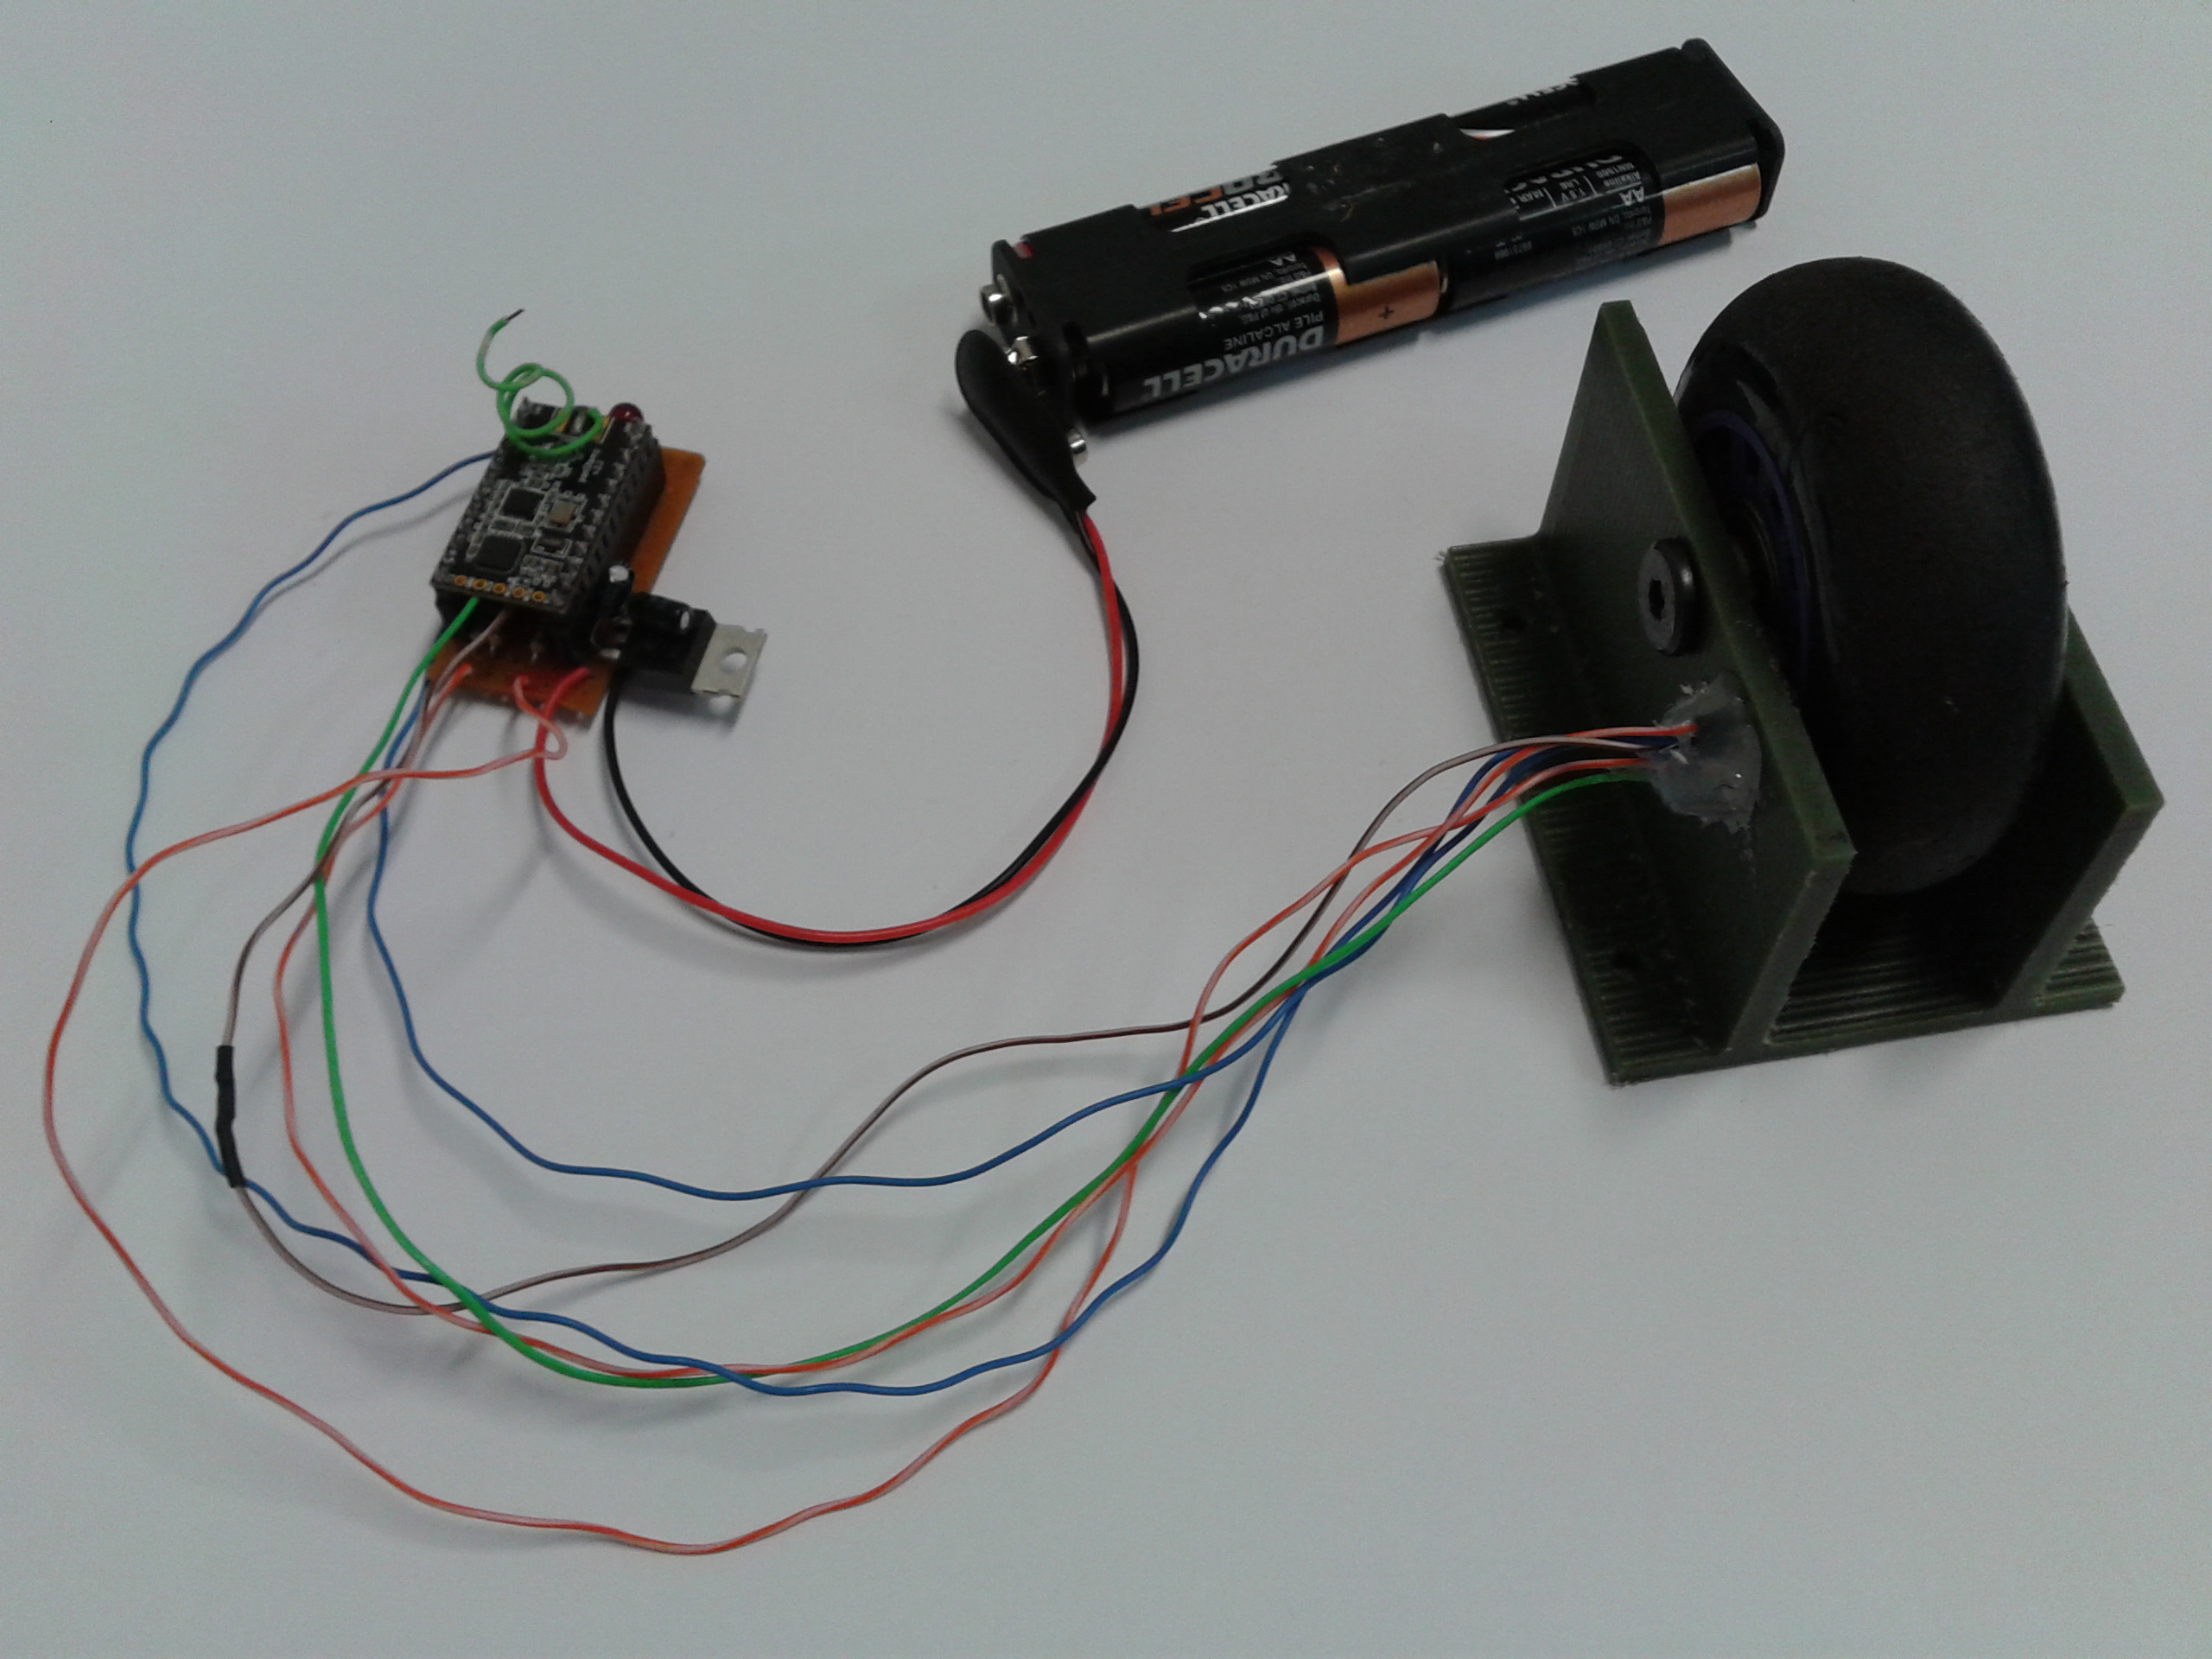
\includegraphics[width= 0.3\textwidth, clip=true  ,keepaspectratio=true]{./pic/wheel.jpg}
 \caption{The wheel and panstamp}
 \label{fig:wheel}
\end{figure}


\subsection{The hall sensor}
The sensor TLI4906 is a Hall Effect Switch, whose output depends on the magnetic field sensed by the chip (see  ). According to the datasheet, a magnetic south pole with a field strength above Bop (typical value 10 mTeslas) turns the output on, whereas a magnetic north pole exceeding Brp (typical value 8.5 mTeslas) turns it off. Figure~\ref{fig:hall-sensor-output}, taken from the datasheet, shows the relationship between the output voltage (named Vq) and the magnetic field sensed by the hall effect ship.

\begin{figure}[h!]
 \centering
 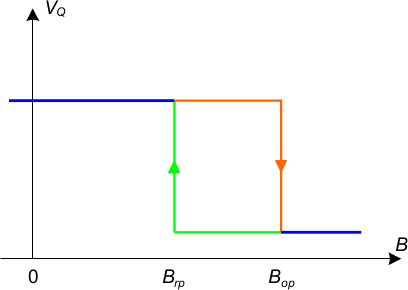
\includegraphics[width= 0.3\textwidth, clip=true  ,keepaspectratio=true]{./graph/hall-sensor-output.png}
 \caption{The hall sensor's output}
 \label{fig:hall-sensor-output}
\end{figure}

 After experimenting with the sensor, we realized that the absence of a magnet in front of the ship also turns the output off. With this property, we could distinguish two possible states:  magnet in front of the chip and no magnet in front of it. Since we were using to hall effect sensors, we could have 4 different states, as shown in Table~\ref{hall-sensor-output}. 
 
 
\begin{table}[h]
  \centering
  \begin{tabular}{ c | c | c | c}
    \hline
    \textbf{Sensor 1} & \textbf{Sensor 2} & \textbf{Vsensor1 } & \textbf{Vsensor2}\\ [0.5ex]    
    \hline
    No magnet & No magnet & 0 & 0 \\
    No magnet & Magnet & 0 & 1\\
    Magnet & No magnet & 1 & 0\\
    Magnet & Magnet & 1 & 1 \\      
    \hline
  \end{tabular}
  \caption[Output voltages in hall effect sensors]%
          {Possible output voltages combinations with the two hall effect sensors}
  \label{hall-sensor-output}
\end{table}

When the wheel rotates, the position of the magnets changes and this alters the combination of outputs of the hall effect sensors. The sequence of different states yields a pattern that can be used to determine the wheel's rotation direction (clockwise or counterclockwise)  In the next section, we describe how the hall effect output signals were processed by the panstamp.

\subsection{Processing the hall effect sensors' signals}

Figure~\ref{fig:Wheel-circuit} shows a simple diagram of the circuit built to determine the wheels direction of rotation. 

\begin{figure}[h!]
 \centering
 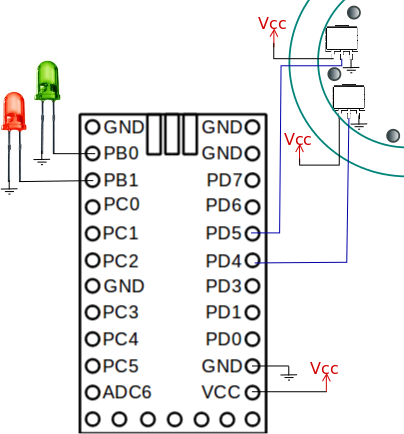
\includegraphics[width= 0.3\textwidth, clip=true  ,keepaspectratio=true]{./graph/wheel-circuit.png}
 \caption{Wheel circuit}
 \label{fig:Wheel-circuit}
\end{figure}

The output pin of each hall effect sensor was connected to a panstamp's digital output pin, namely PD4 and PD5.We configured an interruption, in the panstamp code, that is triggered with each change (rise and fall) in the voltage sensed by pin PD4. In interruption routine, the voltages in PD4 and PD5 were measured and a flag was raised. These voltage measurements were interpreted as binary inputs ('0' or '1') and constituted the trace that reflected the direction of rotation. The location of each magnet in the wheel's spokes was carefully selected to produce clear differences between the clockwise and the counterclockwise trace. The raised flag, mentioned before in the interruption routine, indicated if there was a change or not in the state; that is, if the wheel was rotating or not.

Without the library 'PinChangeInt.h', the only digital pins that can trigger this interruption are digital pins PD2 and PD3. Since the use of PD2 cannot be customized in the Panstamp, we had available just PD3. At the beginning, we thought we needed two interruptions (one triggered by PD4 and another by PD5) but Later, we realized that one interruption sufficed to do the analysis. 
In other words, we could have used pins PD3 and PD4 and configured interruptions with PD3 without the help of the above mentioned library. 

As explained in the arduino official website \cite{arduino}, it is useful to steer a digital input pin to a known state if no input is present. Writing a HIGH value with digitalWrite() in a digital pin, if if the pin is configured as an INPUT, will enable an internal 20K pullup resistor (to Vcc). On the other hand, writing LOW will disable the pullup. In our implementation, adding the internal pullup was fundamental to obtain the right readings of the hall effect sensor's output signals. 

Each time the panstamp detected movement in the wheel, it built a packet and sent it wirelessly to another panstamp that lit up a led strand. Two different packets were sent according to the direction of rotation and the leds in the led strand were lit in a way that reflected the two different directions. For debugging purposes, a led was lit when a certain direction of rotation was detected: the green led indicated clockwise rotation whereas the red one counter-clockwise rotation. 

This mini-project is a simple example of how the hall effect sensors, along with a panstamp, can be used to produce interactive systems. 









\section{Conclusion}
The development of our system required a balanced combination of creativity and technology. First, we analysed already existing projects for public spaces and then some systems where the foot played the main goal. Then, after defining our own concept, we started to explore different possibilities for implementing each necessary component in the concept and chose the options that offered more flexibility and overall utility. 





%TODO do we have sources?
\bibliography{sources}
%\listoftables
%\listoffigures

\end{document}
